\documentclass[12pt]{article} 

%?? paths
\newcommand{\CiteMathPackage}{../../math} 
\newcommand{\CiteReference}{../reference.bib}

%?? packages 
\usepackage{setspace,geometry,fancyvrb,rotating} 
\usepackage{marginnote,datetime,enumitem} 
\usepackage{titlesec,indentfirst} 
\usepackage{amsmath,amsfonts,amssymb,amsthm,mathtools} 
\usepackage{threeparttable,booktabs,adjustbox} 
\usepackage{graphicx,epstopdf,float,soul,subfig} 
\usepackage[toc,page]{appendix} 
\usdate

%?? page setup 
\geometry{scale=0.8} 
\titleformat{\paragraph}[runin]{\itshape}{}{}{}[.] 
\titlelabel{\thetitle.\;} 
\setlength{\parindent}{10pt} 
\setlength{\parskip}{10pt} 
\usepackage{Alegreya} 
\usepackage[T1]{fontenc}
% \usepackage{fourier} % Favorite Font

%?? bibliography 
\usepackage{natbib,fancybox,url,xcolor} 
\definecolor{MyBlue}{rgb}{0,0.2,0.6} 
\definecolor{MyRed}{HTML}{D2042D}
\definecolor{MyGreen}{rgb}{0,0.4,0} 
\definecolor{MyPink}{HTML}{E50379} 
\definecolor{MyOrange}{HTML}{CC5500} 
\definecolor{MyPurple}{HTML}{BF40BF}
\newcommand{\highlightR}[1]{{\emph{\color{MyRed}{#1}}}} 
\newcommand{\highlightB}[1]{{\emph{\color{MyBlue}{#1}}}} 
\newcommand{\highlightP}[1]{{\emph{\color{MyPink}{#1}}}} 
\newcommand{\highlightO}[1]{{\emph{\color{MyOrange}{#1}}}}
\newcommand{\highlightPP}[1]{{\emph{\color{MyPurple}{#1}}}}
\usepackage[bookmarks=true,bookmarksnumbered=true,colorlinks=true,linkcolor=MyGreen,citecolor=MyGreen,filecolor=MyBlue,urlcolor=MyGreen]{hyperref} 
\bibliographystyle{econ}

%?? math and theorem environment 
\theoremstyle{definition} 
\newtheorem{assumption}{Assumption} 
\newtheorem{definition}{Definition} 
\newtheorem{theorem}{Theorem} 
\newtheorem{proposition}{Proposition} 
\newtheorem{lemma}{Lemma} 
\newtheorem{example}{Example} 
\newtheorem{corollary}[theorem]{Corollary} 
\usepackage{mathtools} 
\usepackage{\CiteMathPackage}

\begin{document} 

%??%??%??%??%??%??%??%??%??%??%??%??%??%??%??%??%??%??%??%??%??%?? 
%?? title 
%??%??%??%??%??%??%??%??%??%??%??%??%??%??%??%??%??%??%??%??%??%??

\title{\bf Cyclical Earnings, Career and Employment Transitions, Working Paper, 2022} 
\author{Wenzhi Wang \thanks{This note is written in my pre-doc period at the University of Chicago Booth School of Business.} } 
\date{\today} 
\maketitle 

\citet{carrillo-tudelaCyclicalEarningsCareer2022}

\section{Introduction}

Understanding the nature of earnings risk is important because it impacts individuals' career path decisions, their consumption, savings and investment decisions, and ultimately inequality. \highlightR{In this paper we study the joint behaviour of earnings risk and career changes over the business cycle.} It is well documented that during recessions those individuals who separate directly to another job face lower earnings gains, while those who lose their job suffer larger earnings losses relative to expansions. These patterns are consistent with increasing evidence showing that the distribution of earnings growth exhibits procyclical skewness. \highlightP{Less is known, however, about the type of job mobility that drives cyclical earnings risk and whether the latter is mainly caused by cyclical changes in the returns to mobility (i.e., the earnings change conditional on a transition), cyclical changes in the frequency of job loss and job finding and how workers' mobility decisions interact with them both.} Studying these features is important as they help determine the sources of idiosyncratic earnings risk and why this risk changes over the cycle. Without this understanding it remains difficult to evaluate, for example, whether governments should emphasize labour market policies that aim to bring individuals bask to work quickly over longer duration re-training schemes that help individuals improve the type of their re-employment jobs.

This paper shows that career changes, which we observe as occupational mobility, are the main driver behind the cyclical patterns of the earnings growth distribution. Moreover, it is occupational mobility due to workers' evolving idiosyncratic career prospects rather than occupation-wide productivity differences that makes occupational mobility the more important component. We also show that employer mobility on its own does not contribute as much as occupational mobility in shaping cyclical earnings risk. Further, worsening returns to (idiosyncratic) occupational mobility during recessions explain to a large extent the observe procyclical skewness of earnings changes. Our analysis demonstrate that the sullying effects of recessions are long-lived. They manifest themselves through a collapse of the job ladder, particularly for occupational switchers, and foregone lifetime earnings gains especially for low-paid workers, and through the large lifetime earnings losses faced by high-paid workers who experience forced occupational mobility and poor re-employment outcomes.

To motivate our approach we use the SIPP to construct the annual earnings growth distribution both in the cross-section and over the business cycle. After showing that the earnings growth distribution in our data is also characterized by procyclical skewness and exhibits the same cross-sectional properties as in earlier papers, we present novel evidence showing the importance of occupational mobility driving earnings growth. First we show that, among those individuals who changed employer, there is an increasing relationship between the size of the earnings change (positive or negative) and the probability of an occupational switch. This feature is observed among individuals who made a direct employer transition and among those who changed employers through a spell of unemployment. We then document our main empirical finding. The procyclical skewness of the earnings growth distribution arises mostly from the earnings changes of those individuals who switched employers and occupations at the same time. We find considerably stronger evidence of procyclical skewness among those who made an occupation switch and changed employers directly through a job-to-job transition or through unemployment relative to those who changed employer but did not switch occupation.

To interpret these data patterns, we propose a model of on-the-job search in which a job consists of two dimensions: the employer dimension (where the job is done) and the occupation dimension (the tasks involved in the job). \highlightR{We use this framework to investigate (i) whether cyclical changes in the earnings risk arise from the occupation or from the employer dimension, and (ii) whether the importance of each dimension arises from cyclical changes in returns to mobility or from cyclical changes on worker flows.} A simple decomposition of cyclical changes in observed worker flows and observed earnings changes conditional on flows does not allow us to answer these questions. Observed worker flows reflect worker choices in the face of changing returns, where workers could opt not to reallocate. Observed earnings changes reflect workers' acceptance decisions in the face of alternative employment possibilities, shaped also by the flows, and returns elsewhere. To untangle these forces, we extend the canonical on-the-job search model originally proposed by Burdett (1978)  to a multi-sector business cycle economy with endogenous employer and occupational mobility and  cyclical fluctuations in job loss and job finding probabilities and offer distributions.

In our model, worker and earnings heterogeneity arises principally from two idiosyncratic productivity shocks. Essentially, workers search to improve on the two dimensions of job match quality, occupation- and firm-specific. Occupations are distinguished from one another by their workers' specific match quality and specific human capital as well as occupation-wide productivity differences. A key feature of our framework is that the decision to change employer or occupations is fundamentally different in terms of the workers' information. As is standard in job ladder models, \highlightO{meetings with employers are treated akin to ``inspection'' goods}. Once a worker encounters a firm, he knows enough to make a job acceptance decision. This assumption captures that typically many job interviews reveal enough information to the worker (and firm) to accept or reject the employment offer. As in many multi-sector models following \citet{lucasEquilibriumSearchUnemployment1974}, \highlightO{the decision to change occupations is instead treated akin to an ``experience'' good}. The worker does not know his labour market opportunities before starting the search for a job in the new occupation. This captures that when changing careers workers typically are able ot re-build their employment contacts, learn about new employment opportunities and their job finding prospects only when they start searching for jobs in the new occupation. We show that this structure is able to replicate the data very well.

We use simulated methods of moments to structurally estimate our model. The estimation reveals that workers' endogenous decisions to change employers and occupations with or without intervening spells of unemployment can reproduce the observed cyclical behaviour of the earnings growth distribution, the cyclical behaviour of worker mobility as well as a wide range of cross-sectional patterns that characterize earnings risk and worker mobility. In particular, our model reproduces the (i)  job loss, re-employment and direct employer transition probabilities in the cross-section and over the  business cycle; (ii) the gross occupational mobility patterns among employer stayers and movers in  the cross-section and over the cycle, including the increasing relationship between the size of the earnings change and the probability of an occupation switch; (iii) the bilateral net mobility flows across  occupations; (iv) the earnings growth distributions conditional on workers' employer and occupation  transitions; (v) the cyclical change in the earnings growth distribution, characterized by its procyclical  skewness; and (vi) the cyclical changes of the earnings growth distribution conditional on employer  and occupation transitions, showing that the procyclical skewness arises from simultaneously changes  in employers and occupations.

Our approach allow us to disentangle the separate effects of firm-worker and occupation-worker shocks in explaining the cyclicality of earnings growth. We find that returns to idiosyncratic occupation mobility can explain near the entirety of the difference between the expansion and recessions earnings growth distributions, particularly between the $10$th and $90$th percentiles. Outside this range two major conclusions emerge. At the bottom tail, about $53\%$ of the largest earnings losses we observe in recessions arise from those individuals who lost their jobs and had to change occupations. At the top tail, the more abundant number of opportunities to improve the occupational dimension of a job becomes the more important, and can explain $26\%$ of the largest earnings gains observed in expansions. The remainder is explained by cyclical changes in returns to occupational mobility.

Given the estimates in which both flows and returns respond to the cycle, we investigate the cost of business cycles. In particular, our model implies that cyclical changes in the returns to mobility and probabilities of job loss and job finding affect workers differently based on their positions in the employer and occupation dimensions of the job ladder. For example, by affecting their ability to climb the ladder and their outcomes after falling from it, workers might suffer differently from the sullying effects of recessions. We are interested in whether this sullying effects persists over time. We find that low-paid workers suffer disproportionally more in terms of lifetime earnings during recessions from the reduced opportunities to climb the job ladder and the lower returns to mobility than do high-paid workers. However, we also find that it is high-paid workers who suffer disproportionally more in recessions from job transition through spells of unemployment than low-paid workers. A key result is that these costs arise primarily from the occupation dimension rather than the employer dimension of the a job. This suggests that labour market policies that enable workers to achieve higher returns to occupation mobility through access to higher quality jobs could have a significant impact in reducing cyclical earnings risk and the cost of recessions.

\subsection{Related literature}

\section{The Earnings Growth Distribution}

\subsection{Data}

We use data from the SIPP from the 1990 to 2008 panels, covering the 1990-2013 period. The advantage of using this dataset is that each of its panels follows a large number of workers for up to four years. Within each panel individuals are divided into four rotation groups, where each group is interviewed in waves of four months. At the end of each wave individuals report information on their current and previous employment status, occupations, industries and earnings (hourly wages and hours worked), covering the last four months. Using this information, we define employer, occupation and earnings changes based on a worker's main job\footnote{Since the SIPP records up to two jobs at a time for any individual, we define the main job as the one in which the worker spent the most hours, and break ties using earnings.} for each period.

\paragraph{Labor market flows} Within a panel we identify for each individual whether he/she experienced an employer and/or an occupational transition. Employer changes that occurred without an intervening full month of unemployment are labeled $EE$ transitions and those that occurred through unemployment are labeld $EUE$ transitions. In the latter case, we include all transitions in which the worker returned to employment within the sample, even if the worker did not report actively searching. Since we only consider unemployment spells completed within the survey period, to minimize the potential under-representation of $EUE$ relative to $EE$ transitions we consider only transitions with at least $4$ waves remaining in the panel. $EUE$ transitions, however, would remain affected by our choice to exclude ``temporary recalls,'' as these workers do not seem to face the same reallocation and search frictions as those workers who do not expect to return to their previous employers.

To measure occupation changes we homogenize the occupation classification across SIPP panels  using the crosswalk translation scheme created by IPUMS based on the 1990 Standard Occupational Classification (1990 SOC). We then aggregate the resulting three-digit occupational codes. For our benchmark analysis we use the aggregation based on four task-based occupational categories: Nonroutine Cognitive, Routine Cognitive, Non-routine Manual and Routine Manual. We chose this coarse aggregation to focus on those changes in an individual's line of work that also involve a change in the main tasks performed. We then compare the task-based occupation for a given individual across waves.

For an individual to be labeled an ``employer/occupational stayer'' in a given wave he/she should not have changed either of these dimensions in the previous or in the posterior year relative to this wave. Under this categorization we find that over $75\%$ of the transitions are made up of employer/occupation stayers. The reminder observations contain at least one form of transition. From the latter we label an individual to be an ``employer/occupation mover'' in a given wave when he/she reported a simultaneous employer and occupation change. As mentioned above we distinguish on whether the employer change takes the form of a $EE$ or $EUE$ transition. An individual is labeled as an ``employer stayer / occupation mover'' (``employer mover / occupation stayer'') when we only observe a change in the occupation (employer) dimension of a job.

\paragraph{Earnings} To study earnings we deflate nominal monthly earnings in the SIPP by the Personal Consumption Expenditure price index. Consistent with the recent literature on earnings risk, we use as  our measure of earnings the residuals obtained from regressing log real earnings on a quadratic on potential experience, education and month dummies. After this step we clean reporting errors in the residual earnings data by dropping the bottom and top $2\%$ of the wave-frequency earnings sample and drop imputed earnings. Following the literature we focus on year-to-year earnings growth. We construct annual earnings as the sum of all (residual) monthly earnings observed during the past 12 months. This measure therefore includes any zero earnings associated with the months in which an individual was unemployed. 

For employed workers who do not change employers or occupation and continually at work, earnings growth are computed by comparing the one year earnings to the next. In the case of employer and/or occupation movers, we compare earnings differences in the year prior to a transition to earnings in the year following the wave in which the transition occurred. As mentioned above, some of these transitions include either an $UE$ or $EU$ observation. Because some $EU$ transitions entail reemployment after an unemployment spell that lasted for more than a year and hence these workers are associated with very low or zero earnings, we use the inverse hyperbolic sine differences 
$$
\D_{i, t+1} = \log\of{w_{i, t+1} + \sqrt{w_{i,t+1}^2 + 1}} - \log\of{w_{i, t} + \sqrt{w_{i,t}^2 + 1}}
$$
rather than log differences to compute annual earnings changes, where $w_{i,t}$ denotes the earnings of individual $i$ at time $t$. The inverse hyperbolic sine differences are approximately the same as log differences except in the case of very low and zero  earnings.

\subsection{The earnings distribution in the cross-section and over the cycle}

Figure \ref{carrillo-tudelaCyclicalEarningsCareer2022_fig1}a depicts the distribution of annual earnings growth pooling all years in our sample. Guvenen et al. (2021) shows that key features of this distribution is that it is left skewed and very leptokurtic, with approximately Pareto-distributed tails, hence we plot its log density to better visualize this latter property and show that both properties also are present in our sample. Figure \ref{carrillo-tudelaCyclicalEarningsCareer2022_fig1}b instead presents the earnings growth cdf, where we graph the earnings changes in the y-axis and the quantiles of the distributions in the x-axis. This figure further emphasizes that large earnings changes lie at the bottom and top tails of the distribution. Figure \ref{carrillo-tudelaCyclicalEarningsCareer2022_fig1}c conditions this pdf by whether the earnings change was associated with the worker staying with the same employer or it was obtained through an $EE$ or $EUE$ transition. We observe that employer stayers (who represent the vast majority of workers in our sample) exhibit positive and negative earnings changes that are concentrated around zero. In contrast, employer movers have much more dispersed earnings changes and are primarily the ones behind the distribution's fat tails, as shown in Figure \ref{carrillo-tudelaCyclicalEarningsCareer2022_fig1}a. The large negative earnings changes are mainly due ot workers who experienced $EUE$ transitions, while the large positive earnings changes are due to workers who experienced $EE$ transitions or come back into employment to complete an $EUE$ transition. 

Figure \ref{carrillo-tudelaCyclicalEarningsCareer2022_fig1}d depicts the cyclical changes of the cdf of the earnings growth distribution. This graph is the main data pattern of our analysis. It shows how the earnings growth distribution depicted in Figure \ref{carrillo-tudelaCyclicalEarningsCareer2022_fig1}b changes over the cycle by subtracting for a given quantile (x-axis) the earnings changes in periods of recessions from those in expansions (y-axis). As the median of the expansion and recession cdfs are essentially zero ($0.006$ and $-0.003$, respectively), the bottom half of these distributions represent earnings losses and the top half represent earnings gains. The pronounce U-shape depiced in Figure \ref{carrillo-tudelaCyclicalEarningsCareer2022_fig1}d implies that earnings losses (the left of the distribution) are larger in recessions and earnings gains (the right of the distribution) are larger in expansions. For example, at the 25th percentile of the earnings growth distribution recessions have an earnings loss that is about $4$ percentage points higher than in expansions, while at the 75th percentile expansions have an earnings gain that is about $2$ percentage points higher than in recessions. This property has already been documented by Guvenen et al. (2014) and shows that the annual earnings growth distribution is mainly characterized by its procyclical skewness.

\begin{figure}[H]
    \noindent\caption{Earnings growth distribution in the cross-section and over the cycle}
    \begin{center}
        \resizebox{1\textwidth}{!}{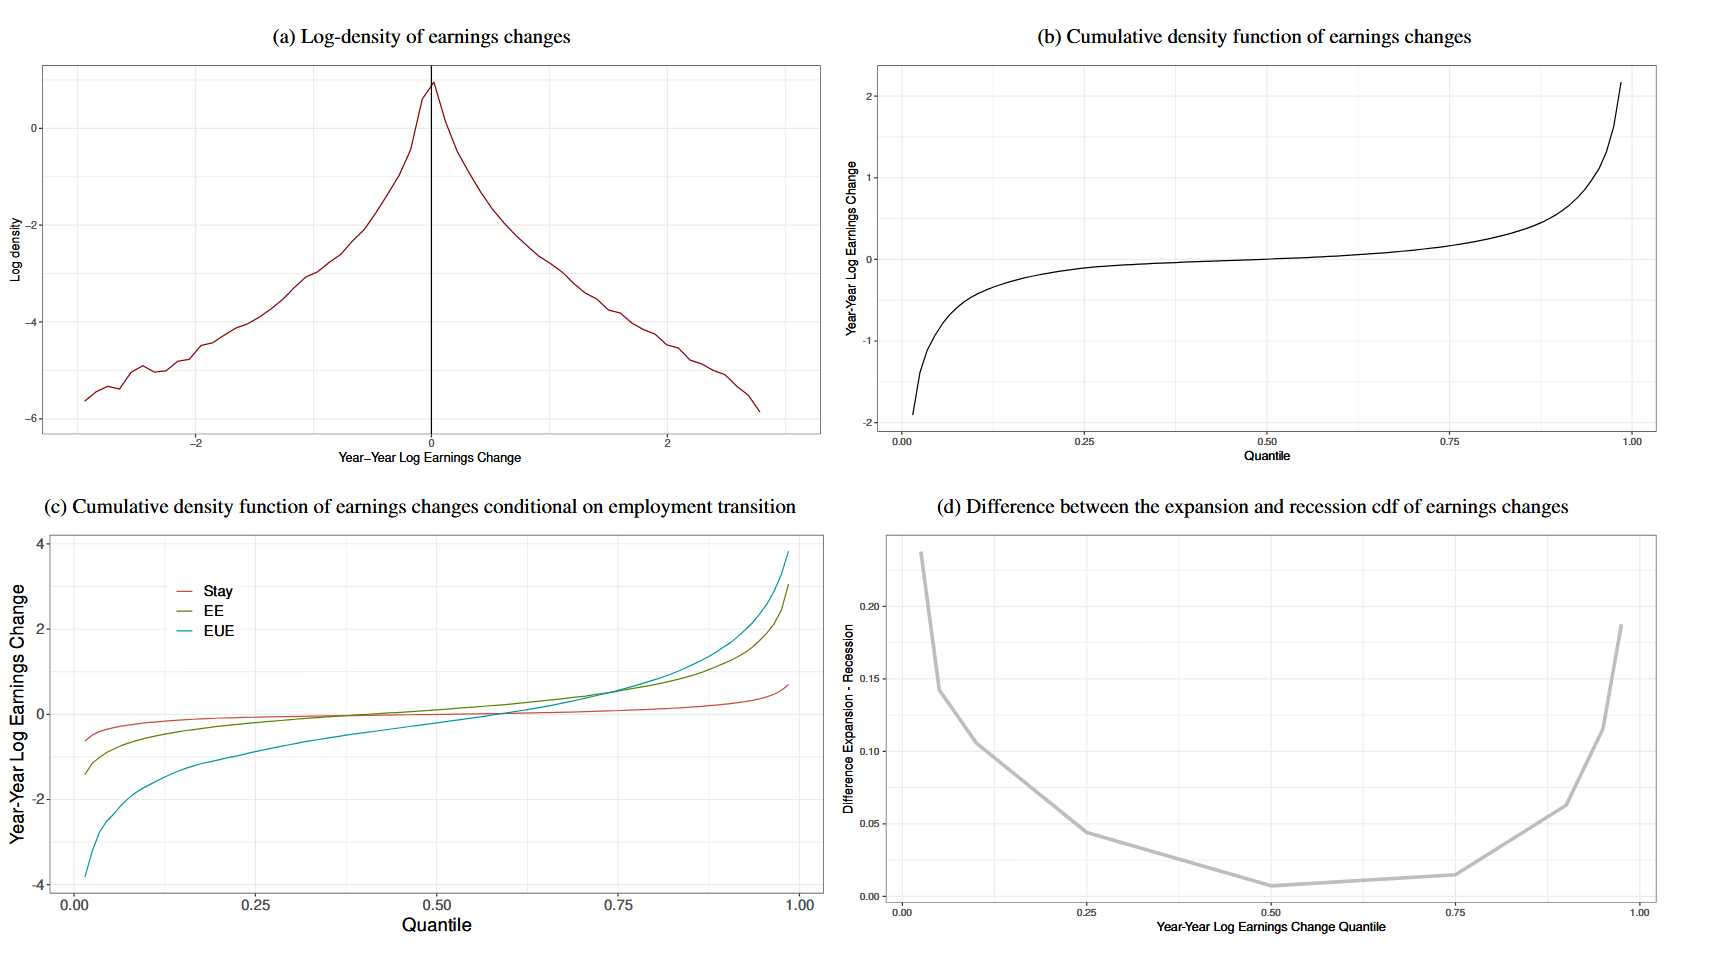
\includegraphics{carrillo-tudelaCyclicalEarningsCareer2022_fig1.png}}
    \end{center}
    \vspace{-20pt}
    {\footnotesize Notes. The annual earnings growth distribution is constructed for the sample period 1990-2013. It is based on residual earnings after controlling for potential experience, education and month dummies. Section 2.1 presents the details of the definition of earnings and worker transitions. Recessions are defined as periods in which the HP-filtered unemployment rate is in the top 20\% of realizations.}
    \label{carrillo-tudelaCyclicalEarningsCareer2022_fig1}
\end{figure}


The key message from Figure \ref{carrillo-tudelaCyclicalEarningsCareer2022_fig1} is therefore that the earnings risk as measured by the earnings growth distribution is characterized by long, thick tails that exhibit very large fluctuations over the business cycle and that this arise from changes in both hourly wages and hours worked. Hence, to understand cyclical changes in the earnings growth distribution, we need to understand its tails and the transitions that comprise it. We now present novel evidence showing the importance of occupational mobility in accounting for the behavior of these tails.

\subsection{The importance of occupational mobility}

\subsubsection{Occupation switching and cross-sectional earnings growth}

\begin{figure}[H]
    \noindent\caption{Earnings growth distribution and occupation mobility}
    \begin{center}
        \resizebox{1\textwidth}{!}{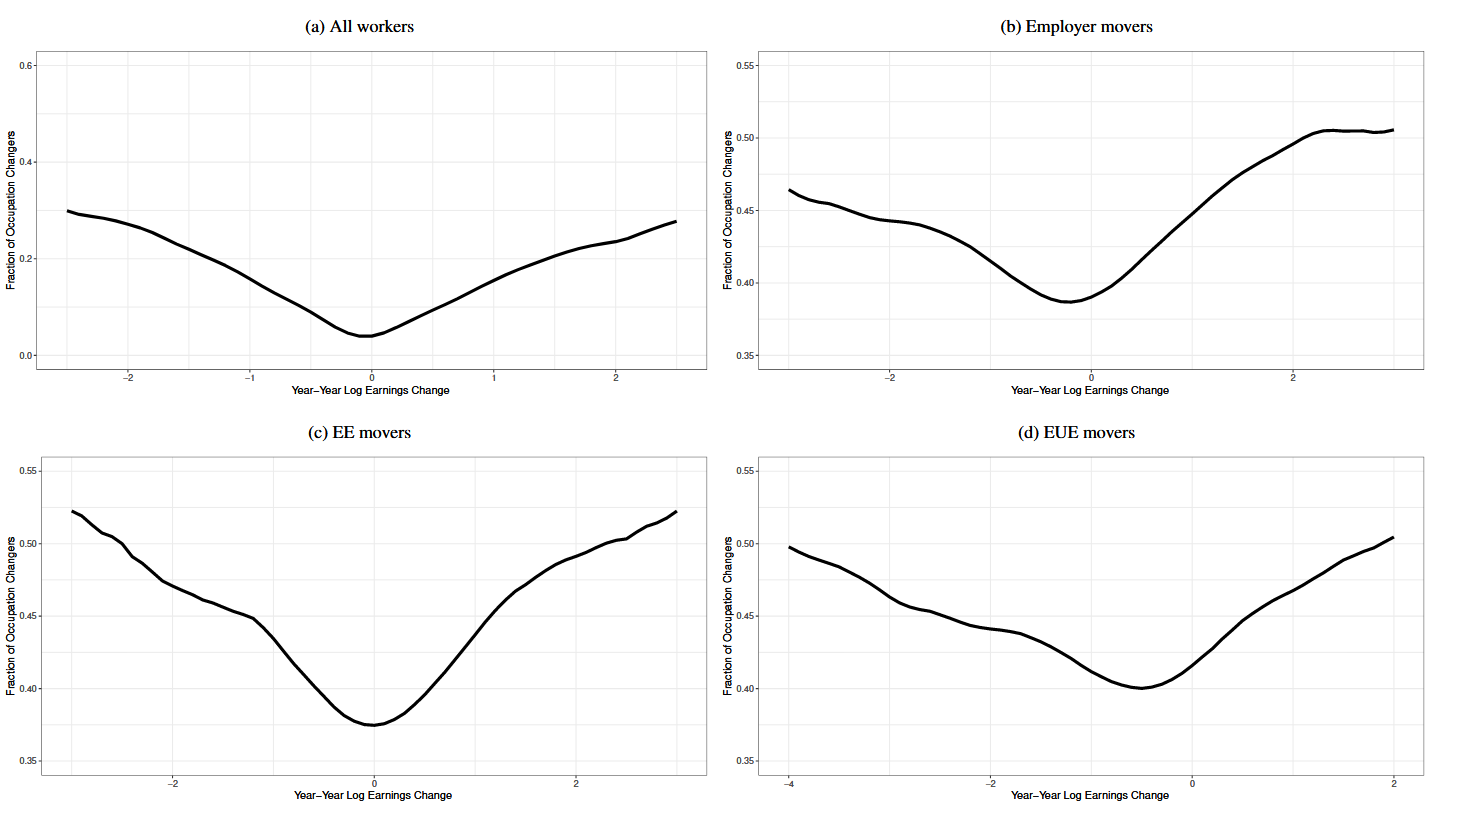
\includegraphics{carrillo-tudelaCyclicalEarningsCareer2022_fig2.png}}
    \end{center}
    \vspace{-20pt}
    {\footnotesize Notes. The probability of occupational change is computed as the proportion of workers with a given earnings change who took a job in a different task-based occupation: Non-routine cognitive, Routine cognitive, Non-routine manual and Routine manual. Earnings changes are based on residual earnings after controlling for potential experience, education and month dummies.}
    \label{carrillo-tudelaCyclicalEarningsCareer2022_fig2}
\end{figure}

Figure \ref{carrillo-tudelaCyclicalEarningsCareer2022_fig2} depicts the probability of an occupational change associated with a given value of earnings growth. Figure \ref{carrillo-tudelaCyclicalEarningsCareer2022_fig2}a shows that when pooling together employer movers and stayers th fat tails of the annual earnings growth distribution depicted in Figure \ref{carrillo-tudelaCyclicalEarningsCareer2022_fig1}a are associated with a high probability of an occupational change. Small earnings changes centered around zero, however, are associated with a much smaller probability of an occupational change. Although the large difference in the probability of an occupational move can be accounted for by the larger propensity to change occupations among employer movers, we observed that the same pattern remains when only considering employer movers, as shown in Figure \ref{carrillo-tudelaCyclicalEarningsCareer2022_fig2}b. Figures \ref{carrillo-tudelaCyclicalEarningsCareer2022_fig2}c and \ref{carrillo-tudelaCyclicalEarningsCareer2022_fig2}d further show that this pattern holds even when analysing separately those individuals who changed employers through an $EE$ or $EUE$ transition. Among $EE$ transitions we observe a near symmetric rise in the probability of occupational mobility and the size of the earnings losses and earnings gains. Among $EUE$ transitions, however, we observe a faster rise in the probability of an occupational change among those workers who had positive earnings growth relative to those with negative earnings growth. This evidence thus shows that large negative or positive earnings changes are associated with a higher propensity to change occupations than smaller earnings changes, even after an employer change has been taken into account.

To investigate further the role of occupational change on the tails of the earnings growth distribution, we calculate the variance of this distribution as the proportion of the sum of squared deviations 
$$
\sum_{K} \sum_{o \in K} \bp{\D w_{o} - \E_{pop}\bs{\D w}}^2
$$
that originates from a group $K$ of workers who share an occupation and employer transition (for example, the set of workers with an $EE$ transition and an occupation switch), and divide it by the overall sum of squared deviations $\sum_{pop} \bp{\D w_{o} - \E_{pop}\bs{\D w}}^2$. We find that occupation movers contribute about $50\%$ of the overall variance of earnings growth, even though the share of occupation movers in our sample is about $17\%$, where the biggest share of this contribution arises from $EUE$ transitions. As we move away from the tails and consider progressively the variance among those between the 0.95-0.05, 0.9-0.1 and 0.75-0.25 percentiles, the contribution of occupation movers and employer movers diminishes, reaching $15\%$ when considering the interquartile range.

\subsubsection{Occupation ladder}

Earnings changes associated with occupational mobility can arise from workers moving from occupations with higher average earnings to occupations with lower average earnings, and vice versa, and from workers changing occupations due to idiosyncratic factors. To investigate the extent of these two sources of earnings growth, we derive conditional occupational earnings averages by estimating an earnings regression, which includes a quadratic for potential experience, dummies for education, gender and race and a set of dummies for occupational categories. We treat the coefficient on the occupational dummies as the occupation-wide earnings effect. For each occupation switcher we then calculate the difference between these coefficients at their source and destination occupation. A positive (negative) difference can be considered as climbing up (falling down) the occupational ladder. We perform this exercise using the 4 task-based categories and the $22$ occupation categories of the two-digit 1990 SOC. Here we present the results based on the task-based categories to keep the benchmark analysis based on the same level of aggregation. 

\begin{figure}[H]
    \noindent\caption{Occupational ladder}
    \begin{center}
        \resizebox{1\textwidth}{!}{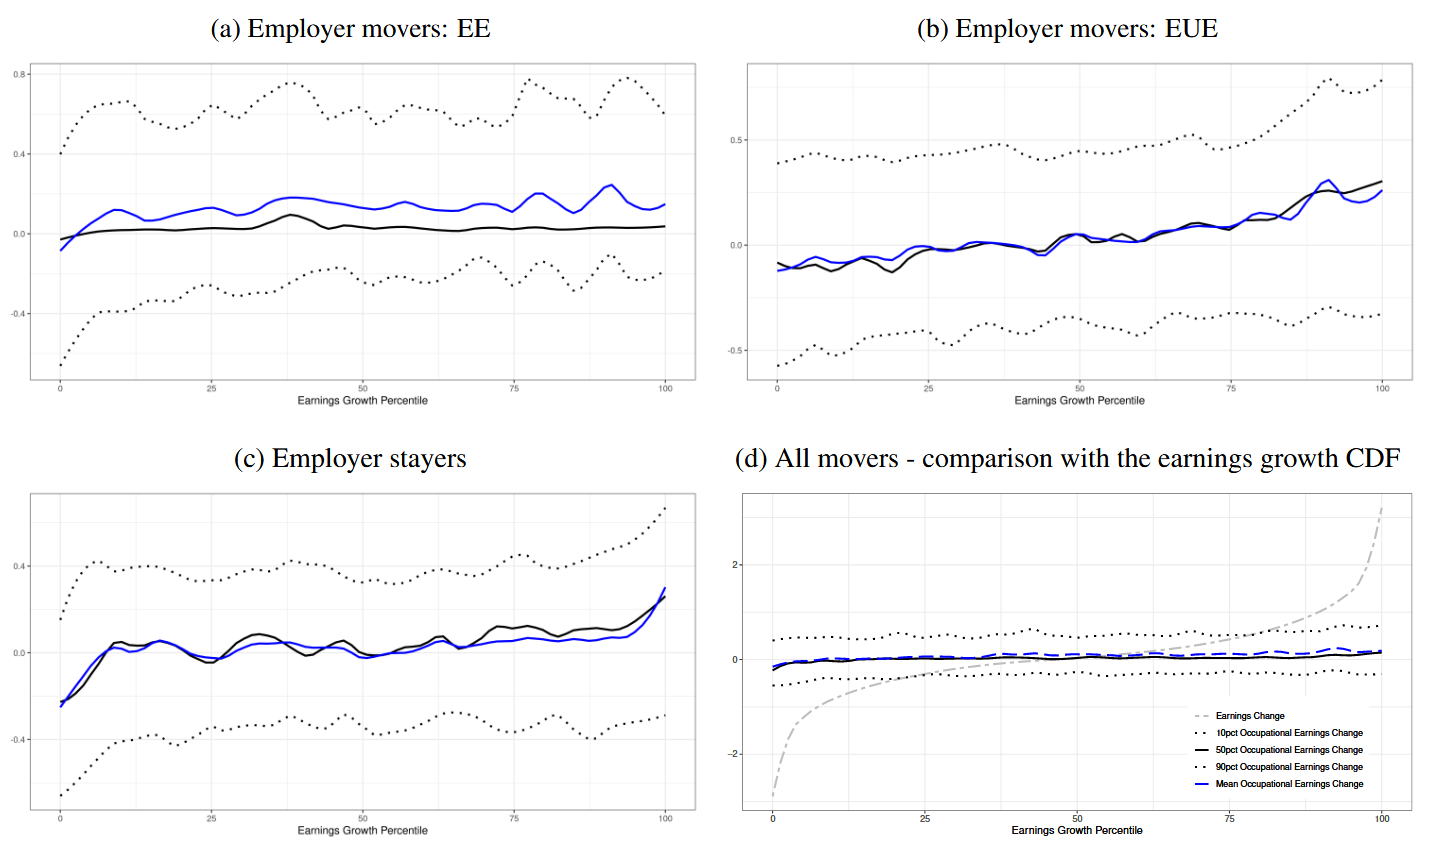
\includegraphics{carrillo-tudelaCyclicalEarningsCareer2022_fig3.png}}
    \end{center}
    \vspace{-20pt}
    {\footnotesize Occupational switchers are ranked by their earnings growth in the horizontal axis. For each rank the vertical axis depicts the mean, median, 90th and 10th percentiles of the distribution of the differences in occupational earnings effects. A similar pattern also holds at two-digit level.}
    \label{carrillo-tudelaCyclicalEarningsCareer2022_fig3}
\end{figure}

Figure \ref{carrillo-tudelaCyclicalEarningsCareer2022_fig3} ranks occupational switchers by their earnings growth (x-axis) and relates each of these workers' rank to the associated distribution of the differences in occupational earnings effects (y-axis). For each rank we show the mean, median, 90th and 10th percentiles of the latter distribution. The bottom and top curves show the sequence of 10th and 90th percentiles obtained from each of these distributions. The middle two curves show the sequence of median and means. This exercise is done for each type of labour market transition. Figure \ref{carrillo-tudelaCyclicalEarningsCareer2022_fig3}b shows an occupation ladder for $EUE$ movers, where the sequence of mean, median, 90th and 10th percentiles are all upward sloping. This implies that workers with higher earnings growth are more likely to move to higher paying occupations. Figure \ref{carrillo-tudelaCyclicalEarningsCareer2022_fig3}c also shows a similar ladder for employer stayers. For $EE$ movers, however, the estimates depicted in Figure \ref{carrillo-tudelaCyclicalEarningsCareer2022_fig3}a only show a noticeable occupational ladder at the mean and the 10th percentile. Although occupational ladders are visible, the key feature of these figures is that these ladders have a very subdued effect on the distribution of changes in the occupational earnings effect. \highlightPP{That is, large earnings changes are associated with movements both up or down the occupational ladder across all types of labour market transitions.} Further, Figure \ref{carrillo-tudelaCyclicalEarningsCareer2022_fig3}d shows that the magnitude of the difference in the occupation effects is small compared to the magnitude of earnings growth. It does so by depicting comparing the distribution of changes in occupational earnings effects among all occupation movers to the CDF of the cross-sectional earnings growth distribution. \highlightP{These findings suggest that the more important factor for occupational change is the idiosyncratic motive rather than average occupation-wide earnings differences when explaining the earnings growth distribution.}

\subsubsection{Occupation switching and cyclical earnings growth}

To highlight the role of occupation mobility in the cyclical change of earnings growth, Figure \ref{carrillo-tudelaCyclicalEarningsCareer2022_fig4}a decomposes the difference in the earnings growth distribution between expansions and recessions by whether workers were occupational movers or stayers conditioning on employer change. As in Figure 1d we subtract the expansion from the recession earnings growth distribution.

\begin{figure}[H]
    \noindent\caption{Cyclical earnings growth distribution by occupation mobility}
    \begin{center}
        \resizebox{1\textwidth}{!}{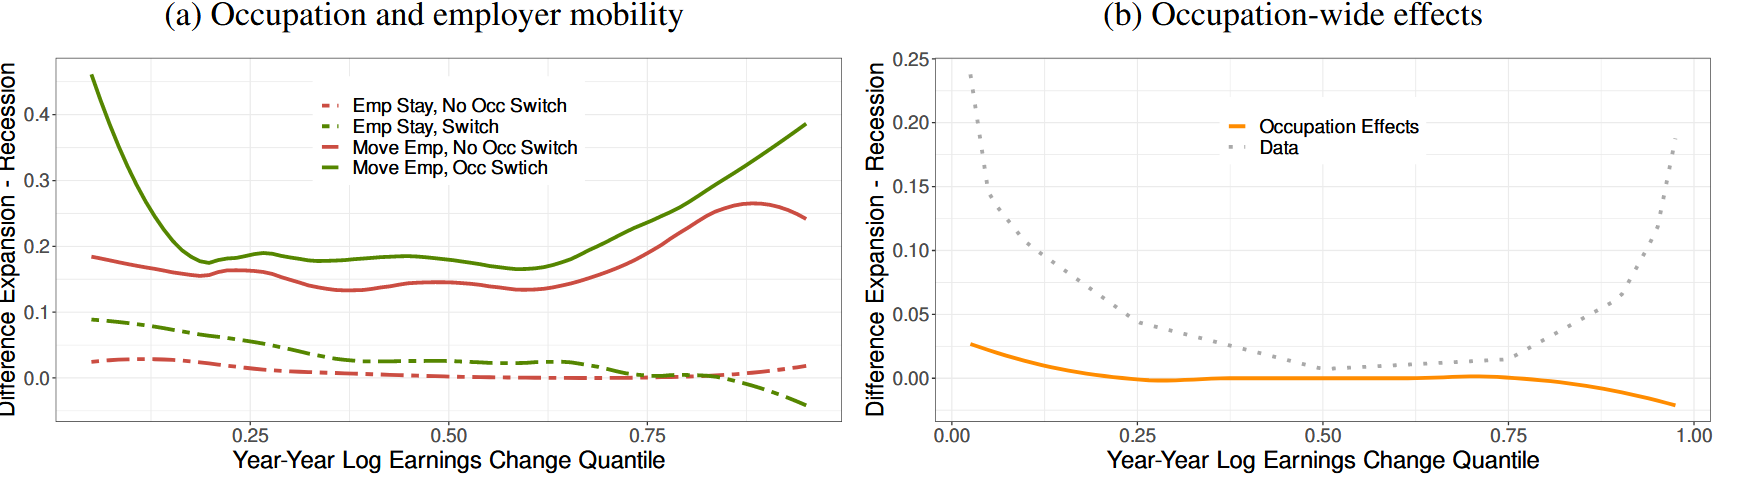
\includegraphics{carrillo-tudelaCyclicalEarningsCareer2022_fig4.png}}
    \end{center}
    \vspace{-20pt}
    {\footnotesize Notes. In the left panel the cyclical change in the annual earnings growth distribution is constructed separately for those workers who (i) simultaneously change employers and occupations, (ii) change employers but did not change occupations, (iii) did not change employers and chance occupations, (iv) or did not change either of these dimensions. In the right panel the cyclical changes in earnings are computed based on changes in the estimated occupation fixed effects. This is done separately for expansion and recessions. In either case we fix the quantile of the distribution along the horizontal axis and we subtract the associated expansion from the recession earnings growth along the vertical axis.}
    \label{carrillo-tudelaCyclicalEarningsCareer2022_fig4}
\end{figure}

Among employer stayers we observe that occupation movers have larger earnings losses during recessions than occupation stayers. However, these losses are modest, increasing only slightly towards the bottom end of the distribution. These workers also exhibit larger and modest earnings gains in expansions relative to occupational stayers. At the very top of the distribution (above the third quartile) we observe the opposite pattern. In recessions those who changed occupations within the same employer receive larger earnings gains relative to occupation stayers. Overall this leads to the earnings growth distribution of employer stayers/occupation movers to exhibit countercyclical variance. For occupational/employer stayers we instead observe a slight level-change between recession and expansions, whereby earnings losses in recessions are of similar magnitude as earnings gains in expansions.

In contrast, employer movers who also changed their occupation exhibit larger losses in recessions relative to occupation stayers and these losses become much larger at the bottom end of the distribution. Further, they also exhibit larger gains in expansions, which also become even larger at the top end of the distribution. These cyclical features create a U-shape pattern that mimics quite closely that of the overall earnings growth distribution (Figure \ref{carrillo-tudelaCyclicalEarningsCareer2022_fig1}d) and implies that the earnings growth distribution of employer/occupation movers is characterized by procyclical skewness. Among those who changed employers but did not change occupations we observe a nearly constant increase in earnings losses during recessions, while an increasing pattern of larger earnings gains during expansions. That is, these workers do not seem to experience an increase in the downside earnings risk of changing employers during recessions.

Figure \ref{carrillo-tudelaCyclicalEarningsCareer2022_fig4}b investigates whether the joint effect of occupation/employer mobility in determining the procyclical skewness of the earnings growth distribution is due to workers moving more often  to better or worse occupations at different points of the business cycle. We use the same procedure as described above to generate occupation-wide fixed effects and compute the difference in the fixed effects associated with workers switching occupations. We do this separately for expansions and recessions and then subtract the difference at each quantile. The figure shows that occupation-wide earnings differences do not seem to explain the observed cyclical changes in the earnings growth distribution. Instead, the figure points to earnings change due to idiosyncratic occupational mobility in explaining procyclical skewness.


\begin{figure}[H]
    \noindent\caption{The cyclicality of earnings growth - employer movers and occupation movers/stayers}
    \begin{center}
        \resizebox{1\textwidth}{!}{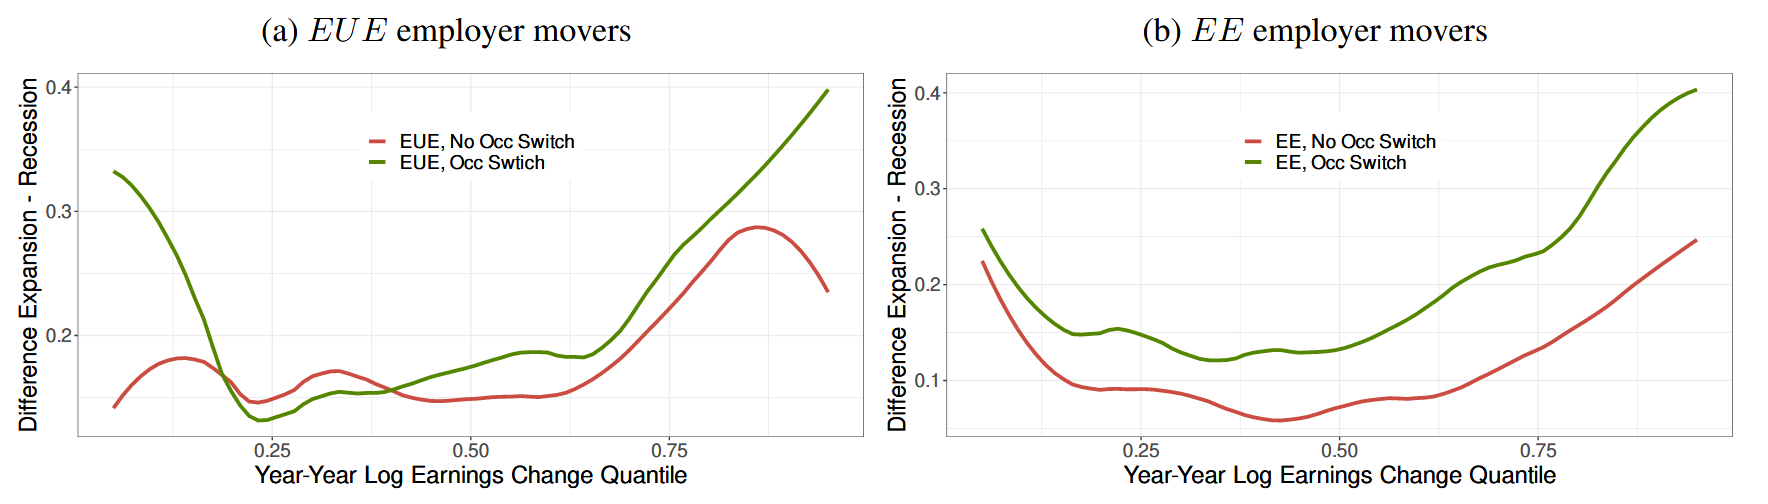
\includegraphics{carrillo-tudelaCyclicalEarningsCareer2022_fig5.png}}
    \end{center}
    \vspace{-20pt}
    {\footnotesize Notes. Among those who change employers and conditional on the type of employer transition ($EUE$ or $EE$), the cyclical change in the annual earnings growth distribution is constructed separately for those workers who simultaneously change occupations and for those who did not change occupations. For each case we fix the quantile of the distribution along the horizontal axis and we subtract the associated expansion from the recession earnings growth along the vertical axis. Earnings changes are based on residual earnings after controlling for potential experience, education and month dummies.}
    \label{carrillo-tudelaCyclicalEarningsCareer2022_fig5}
\end{figure}

Figure \ref{carrillo-tudelaCyclicalEarningsCareer2022_fig5} decomposes the cyclicality of the earnings growth distribution among employer movers  depicted in Figure \ref{carrillo-tudelaCyclicalEarningsCareer2022_fig4}a by the type of transition: $EUE$ or $EE$. It is clear from this figure that those who simultaneously changed their occupation and employer either through an $EUE$ or $EE$ transition exhibit earnings growth distributions characterized by their procyclical skewness. Perhaps unsurprisingly, during recessions the earnings losses among those occupation/$EUE$ movers are more pronounced than among occupation/$EE$ movers. During expansions, however, both type of transitions lead to similar increases in earnings gains. Among employer movers/occupation stayers only those who experienced an $EE$ transition are the ones that exhibit an earnings growth distribution characterized by procyclical skewness. Those who changed employers through an $EUE$ transitions exhibit a level change in their earnings losses during recessions, but an increase in earnings gains during expansions. Since we observe more $EUE$ transitions during recessions, these pattern dominates the cyclical change of the downside earnings risk of the earnings growth distribution among employer movers/occupation stayers as depicted in Figure \ref{carrillo-tudelaCyclicalEarningsCareer2022_fig4}a.

Taken together the above evidence strongly suggests that the procyclical skewness observed in the overall earnings growth distribution depicted in Figure \ref{carrillo-tudelaCyclicalEarningsCareer2022_fig1}d can be traced back to a combination of larger recessionary earnings losses among those occupation movers who changed employers through $EUE$ (and to a lesser extent $EE$) transitions, and the larger earnings gains during expansions among those occupational movers who changed employers through either $EUE$ or $EE$ transitions. Further, these cyclical changes in earnings are a result of changes in both hourly wages and hours worked among employer/occupation movers. Underlying these transitions we find a prominent role for idiosyncratic occupation/employer mobility and not occupation-wide differences.




\bibliography{\CiteReference} 

\end{document}